\documentclass[11pt]{amsart}

% Standard letter size paper with 1inch margins
\usepackage[letterpaper, margin=1in]{geometry}

% Useful packages 
\usepackage{amsmath, amssymb, amsthm, amsaddr}
\usepackage{enumerate, subcaption, graphicx, hyperref}


\title{Graphical Semi-Supervised Learning}
\author{Lucas Cassin Cruz Burke} % first and last name

\address{Department of Applied Mathematics, University of Washington, Seattle, WA 
\\ \texttt{lccburke@uw.edu}}

\date{\today} % you can also just type the date instead of "\today"

\begin{document}

\maketitle 

\begin{abstract}
    This report presents an exploration of semi-supervised learning (SSL) techniques, specifically focusing on Laplacian-based methods and their formulation within the Reproducing Kernel Hilbert Space (RKHS) framework. The theoretical underpinnings of our methodology, including the Probit model, Gaussian Random Fields (GRFs) with the Matérn kernel, and Reproducing Kernel Hilbert Spaces (RKHS), are discussed. We implement and compare the Laplace learning and Poisson learning methods in a simple binary classification problem using the \textit{graphlearning} Python package. Our analysis also investigates the effects of varying kernel parameters and label rates on the accuracy of the classifiers. 
\end{abstract}

\section{Introduction and Overview}\label{sec:Introduction}

With the rise of "big data", the ability to label data in a way that is efficient and cost-effective has become a critical challenge. A common scenario in machine learning is having access to a large amount of unlabeled data and a relatively small amount of labeled data. Traditional supervised learning methods, which rely heavily on labeled data, tend to encounter a bottleneck under these circumstances. Semi-Supervised Learning (SSL) has emerged as an important solution to this problem \cite{zhu2005}.

SSL bridges the gap between unsupervised and supervised learning by exploiting the underlying structure of unlabeled data to extract additional information than what is initially available from the labeled data alone. The main hypothesis of SSL is that similar inputs should yield similar outputs. Therefore, if a pattern or structure can be identified in the unlabeled data, it can be utilized to predict the labels of these data points.

One particular approach to SSL is graphical methods, where the data points are represented as a graph. The goal is to predict the labels of the unknown data points using the graph's structure and the labels of the known data points. Graph-based methods build upon the assumption that points close to each other in the feature space should share similar labels. In the context of the graphical representation, this translates to nodes close to each other in the graph. A popular technique in this category involves the use of a Graph Laplacian, a matrix that provides a measure of the graph's structure \cite{amath563}.

In this report, we focus on formulating Laplacian based SSL methods within the Reproducing Kernel Hilbert Space (RKHS) framework. The RKHS methods offer a promising approach to handle the inherent complexities in real-world data. We investigate the connection between Positive Definite Symmetric (PDS) kernels, such as the Matérn family, and the Green’s function of elliptic differential operators to construct our framework. The choice of kernel can have significant implications for the performance of our SSL algorithm, and thus, we will also explore its impact.

\section{Theoretical Foundations}\label{sec:theory}

This section presents an in-depth exploration of the theoretical principles that form the backbone of our approach, which integrates the Probit model, Gaussian Random Fields (GRFs) utilizing the Matérn kernel, and Reproducing Kernel Hilbert Spaces (RKHS).

\subsection{The Probit Model}\label{sec:probit_model}

The Probit model is a binary classification model which posits the existence of a latent variable, obeying a Gaussian distribution, linked to each data point. \cite{hoffman2020} A binary outcome emerges when a threshold function— the Cumulative Distribution Function (CDF) of the standard Normal distribution— is applied to this latent variable. The mathematical expression of this model is as follows:

\begin{align*}
y_j = \operatorname{sign} (f(\mathbf x_j) + \varepsilon_j), \quad \varepsilon_j \sim \mathcal N(0, \sigma^2)
\end{align*}

One-hot encoding techniques enable the Probit model to be extended to multi-class classification tasks. These techniques convert categorical variables into a binary vector form. This model's straightforwardness and wide-ranging utility make it especially potent for binary classification tasks.

In addition, the Probit model frequently corresponds with a loss function known as the Probit loss. This function quantifies the discrepancy between the predicted and actual binary outcomes and can be expressed mathematically as:

\begin{align*}
L(y, f(x)) = \Phi(-yf(x)),
\end{align*}

Here, $\Phi$ denotes the CDF of the standard normal distribution, while $y$ and $f(x)$ represent the true and predicted labels, respectively.

\subsection{Graph-Based Methodologies and the Graph Laplacian}\label{sec:graph_laplacian}

Graph-based methods have exhibited strong efficacy in semi-supervised learning. These methods construct a graph $G = (\mathbf{X}, \mathbf{W})$ from input data, where $\mathbf{X}$ signifies the set of data points (vertices), and $\mathbf{W}$ is the weight matrix illustrating relationships between these points. Each element $W_{ij}$ in the weight matrix indicates the similarity between points $i$ and $j$.

The Graph Laplacian, symbolized by $\Delta$, is formulated as $\Delta = \mathbf{D} - \mathbf{W}$, with $\mathbf{D}$ being the degree matrix—a diagonal matrix whose entries represent the sum of the corresponding row's weights in $\mathbf{W}$. The Graph Laplacian captures the graph's structure and serves as a discretized version of the continuous Laplace operator, thereby playing a pivotal role in numerous algorithms, including clustering, dimensionality reduction, and semi-supervised learning.

\subsection{Gaussian Random Fields, the Matérn Kernel, and SPDEs}\label{sec:grf_matern_spde}

A Gaussian Random Field (GRF), a multidimensional extension of a Gaussian process, is a set of random variables wherein any finite subset obeys a multivariate Gaussian distribution. When combined with a Gaussian process prior on the latent variables, the Probit model acquires intriguing characteristics. A Gaussian process is fully defined by its mean and covariance function, which is usually specified by a positive definite (PD) kernel function, such as the Gaussian radial basis function, or its generalization, the Matérn kernel:

$$C_\nu (d) = \sigma^2 \frac{2^{1-\nu}}{\Gamma(\nu)}\left( \sqrt{2\nu} \frac{d}{\rho} \right)^\nu K_\nu \left( \sqrt{2 \nu} \frac{d}{\rho}\right)$$

The Matérn kernel belongs to a family of stationary covariance functions parameterized by a smoothness parameter $\nu$. This parameter regulates the number of continuous derivatives of the realizations, thereby controlling the degree of regularity within the function space. The Matérn kernel evolves into the Gaussian kernel as the smoothness parameter approaches infinity, and condenses to the exponential kernel when the parameter is 0.5.

By considering a Stochastic Partial Differential Equation (SPDE) with a Matérn operator, we can establish a link between Gaussian random fields and SPDEs. The solution to the SPDE yields a Gaussian field with a Matérn covariance function. This reveals that the covariance function of the Gaussian field corresponds to the Green's function of the Matérn operator. \cite{sanzalonso2023}

This relationship enables us to approximate the continuous Laplacian operator using the discrete Laplacian, paving the way for methods like the heat equation on the graph. This motivates the use of graph-based methodologies and the Laplace/Poisson equations in subsequent parts of this report.

\subsection{Reproducing Kernel Hilbert Spaces (RKHS)}\label{sec:rkhs}

The theory of Reproducing Kernel Hilbert Spaces (RKHS) forms a crucial part of our theoretical structure. As the Matérn kernel is positive definite, we can leverage it to define an RKHS—a space of functions where point evaluation becomes a continuous linear functional. Within this context, the Probit model solution can be articulated using the reproducing property. \cite{amath563}

We recast the Probit problem within an RKHS as follows:

\begin{align*}
\mathbf f^* = \operatorname{arg\,min}_{f \in \mathbb R^M} \left\{ - \sum_{j=1}^N \log \Psi (f_j y_j) + \beta \mathbf f^T C \mathbf f \right\}
\end{align*}

Here, $C = \left( \Delta + \tau^2 I \right)^{-\alpha/2}$ and $\Delta = D - W$ represents the graph Laplacian, employed as a regularization term in this model.

Since $C$ is strictly positive definite symmetric, it serves to define an RKHS. Applying the reproducing property of the RKHS, one can show

\begin{align*}
\mathbf f^* = C(:, 1:N)C(1:N, 1:N)^{-1}\mathbf z^,
\end{align*}

where

\begin{align*}
\mathbf z^* = \operatorname{arg\,min}_{\mathbf z \in \mathbb R^N} \left\{-\sum_{j=1}^N \log \Psi (y_j z_j) + \beta \mathbf z^T C(1:N, 1:N)^{-1} \mathbf z \right\}.
\end{align*}

This approach diverges from graph-based methodologies as it harnesses the properties of the RKHS, thereby anchoring our methodology to a solid theoretical framework.

The theoretical groundwork laid out in this section will guide the computational algorithms and results that we will introduce in subsequent sections of this report, as we explore various graph-based SSL algorithms. 

\section{Algorithm Implementation and Development}

We will be using the \textit{graphlearning} Python package developed by Jeff Calder \cite{graphlearning}, which greatly simplifies algorithm implementation and benchmarking. We implement the following algorithms and compare their performance in a simple toy model classification problem.  

\begin{itemize}
    \item \textbf{Laplace Learning:} One of the most extensively utilized techniques in graph-based semi-supervised learning, Laplace learning pursues a graph harmonic function that extrapolates the provided labels. This process shares similarities with uncovering the steady state solution to the heat equation on the graph with Dirichlet boundary conditions applied to the labeled points \cite{pmlr-v119-calder20a}.

    Despite Laplace learning's demonstrated effectiveness across a multitude of applications, challenges arise in scenarios with extremely low label rates. Under such circumstances, label values are inadequately propagated, leading to localized spikes in proximity to the labeled points and nearly constant values far removed from the labeled points. Consequently, more recent methods have been proposed to rectify this degradation in performance for smaller label rates, such as $p$-Laplace learning and Poisson learning. \cite{pmlr-v119-calder20a}

    \item \textbf{Poisson Learning:} Poisson learning, a method closely aligned with Laplace learning, seeks to enhance label propagation and stability. This is achieved by supplanting the assignment of label values at the training points with heat sources and sinks. By this method Poisson learning aims to counteract the performance deterioration observed in Laplace learning when label rates are low. \cite{pmlr-v119-calder20a}.
\end{itemize}

\section{Computational Results}\label{sec:results}


\subsection{Label propagation and convergence}
To demonstrate the different convergence and label propagation properties of the Laplace learning and Poisson learning methods we applied them both to an identical binary classification problem with two labeled training points. 

Figures \ref{laplace_propagation} and \ref{poisson_propagation} visualize the label propagation behavior for the Laplace and Poisson methods after 10, 100, 1000, and 10,000 finite difference steps in the graph Laplace and Poisson equations, respectively. We see that for this example the Laplace method converges faster, while the Poisson method takes time to "warm up". After 10,000 steps both methods converge to the same accuracy, but we can see that the Poisson method results in more opinionated classification, and that label values propagate further from their source as compared with the Laplace method. 

\begin{figure}[h!]
    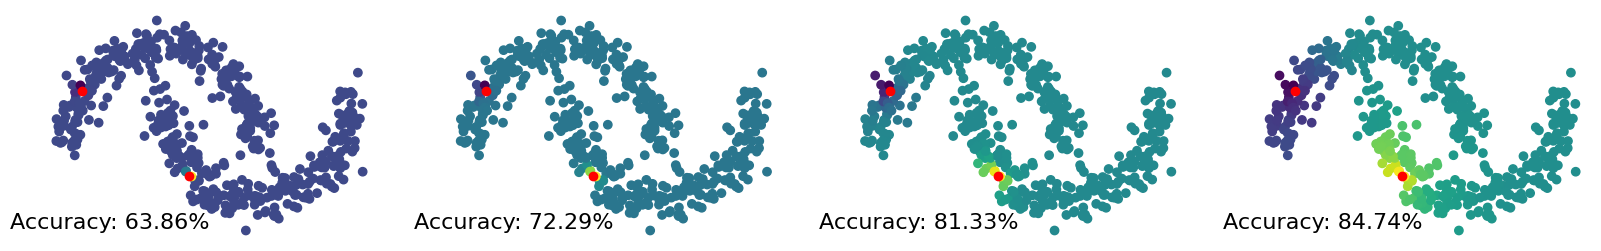
\includegraphics[width=15cm]{Figs/LaplaceSSL.png}
    \caption{Label propagation in Probit model using Laplace method.}
    \label{laplace_propagation}
\end{figure}

\begin{figure}[h!]
    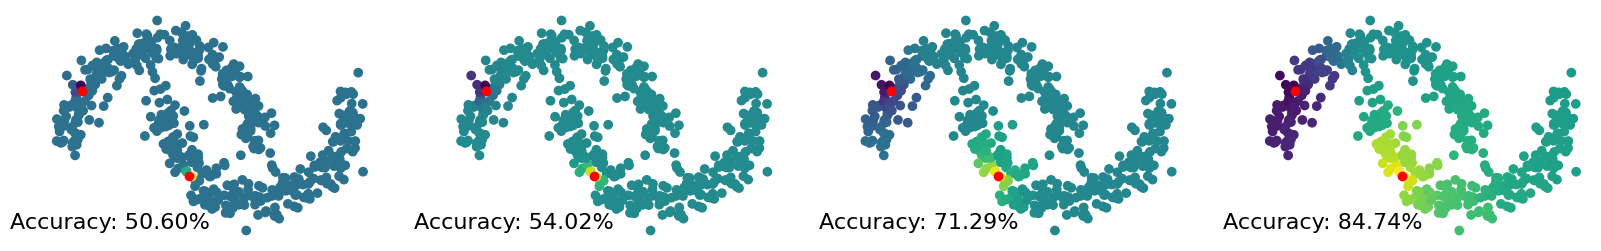
\includegraphics[width=15cm]{Figs/PoissonSSL.png}
    \caption{Label propagation in Probit model using Poisson method.}
    \label{poisson_propagation}
\end{figure}

\subsection{Effect of kernel parameters}

To investigate the effect of kernel parameters on label propagation we defined Matérn kernels using a variety of different smoothness parameters $\nu$ and length scale parameters $\sigma$. We then applied the Laplace method with Gaussian KNN (K=5) and observed the effect of these parameters on the resulting distribution.

\begin{figure}[h]
    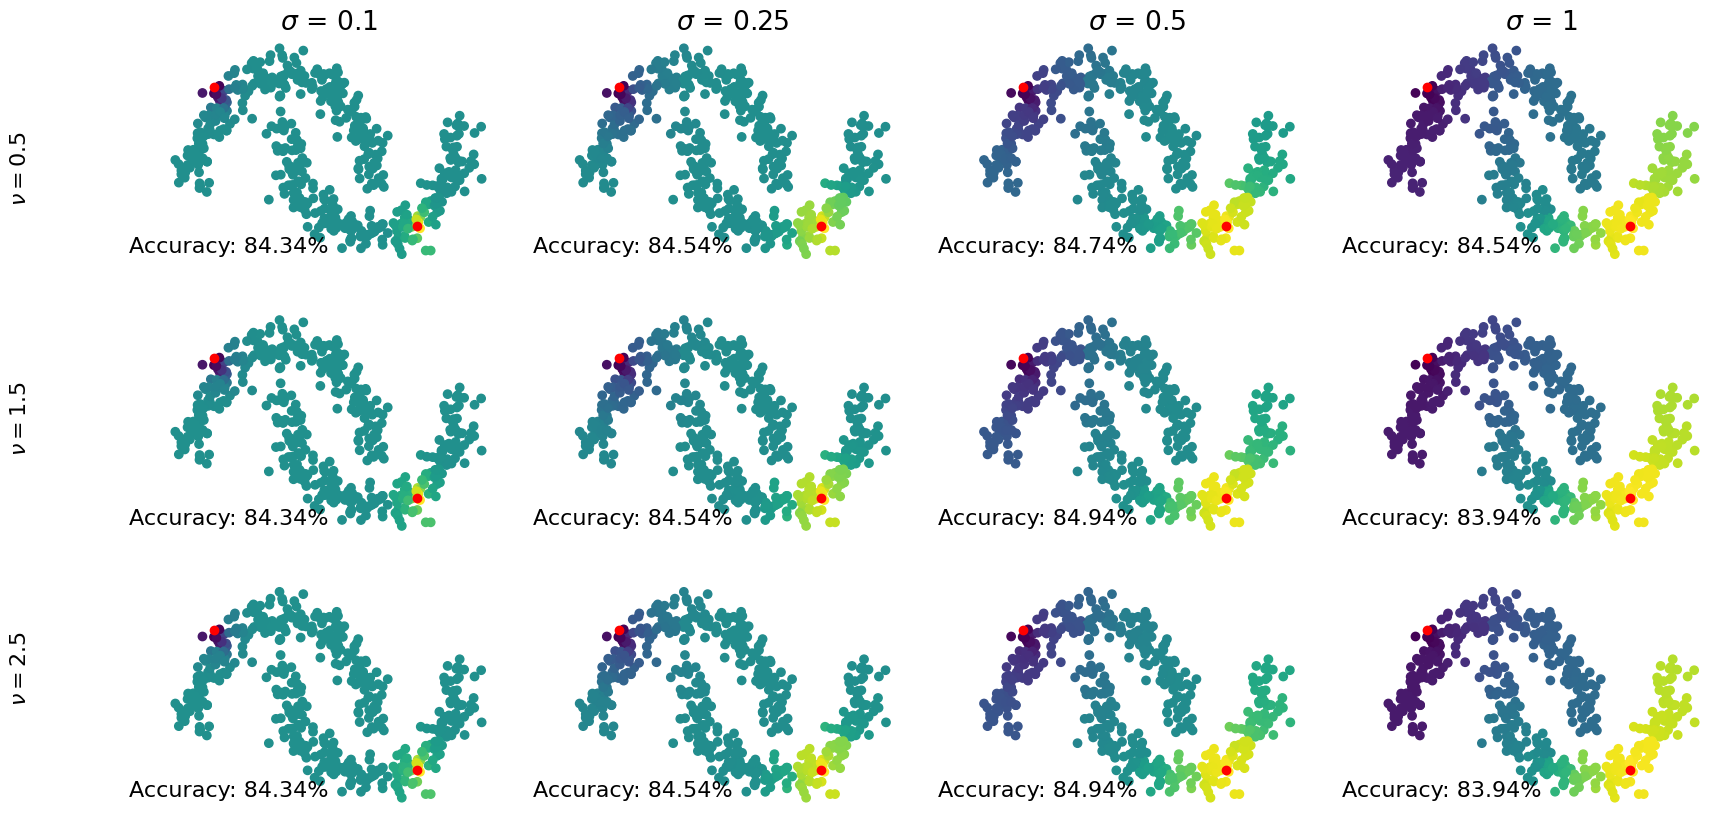
\includegraphics[width=15cm]{Figs/laplace_cv.png}
    \caption{Laplace method solve for differt values of $\nu$ and $\sigma$.}
    \label{laplace_cv}
\end{figure}

As can be seen in Figure \ref{laplace_cv}, the effect of the smoothness parameter $\nu$ is nearly negligible for this simple problem, making only a slight difference for the case where $\sigma=1$. In a problem such as this where the data distribution is quite smooth this is not particularly surprising. 

On the other hand the $\sigma$ parameter has a much more pronounced effect, with higher values corresponding to labels propagating further. 

\subsection{Effect of label rate}

Figure \ref{labelrate} shows the relative performance of the Laplace and Poisson learning methods for different numbers of labeled datapoints. We expected the Poisson method to outperform the Laplace method for low label rates, and indeed we see that for $<5$ labeled points the Poisson method outperforms the Laplace method. However for larger label rates the Laplace method performance continues increasing with more labels while the Poisson method tapers out near 88\% accuracy, indicating that the Laplace method is superior for problems with a more labeled data available. 

\begin{figure}[h!]
    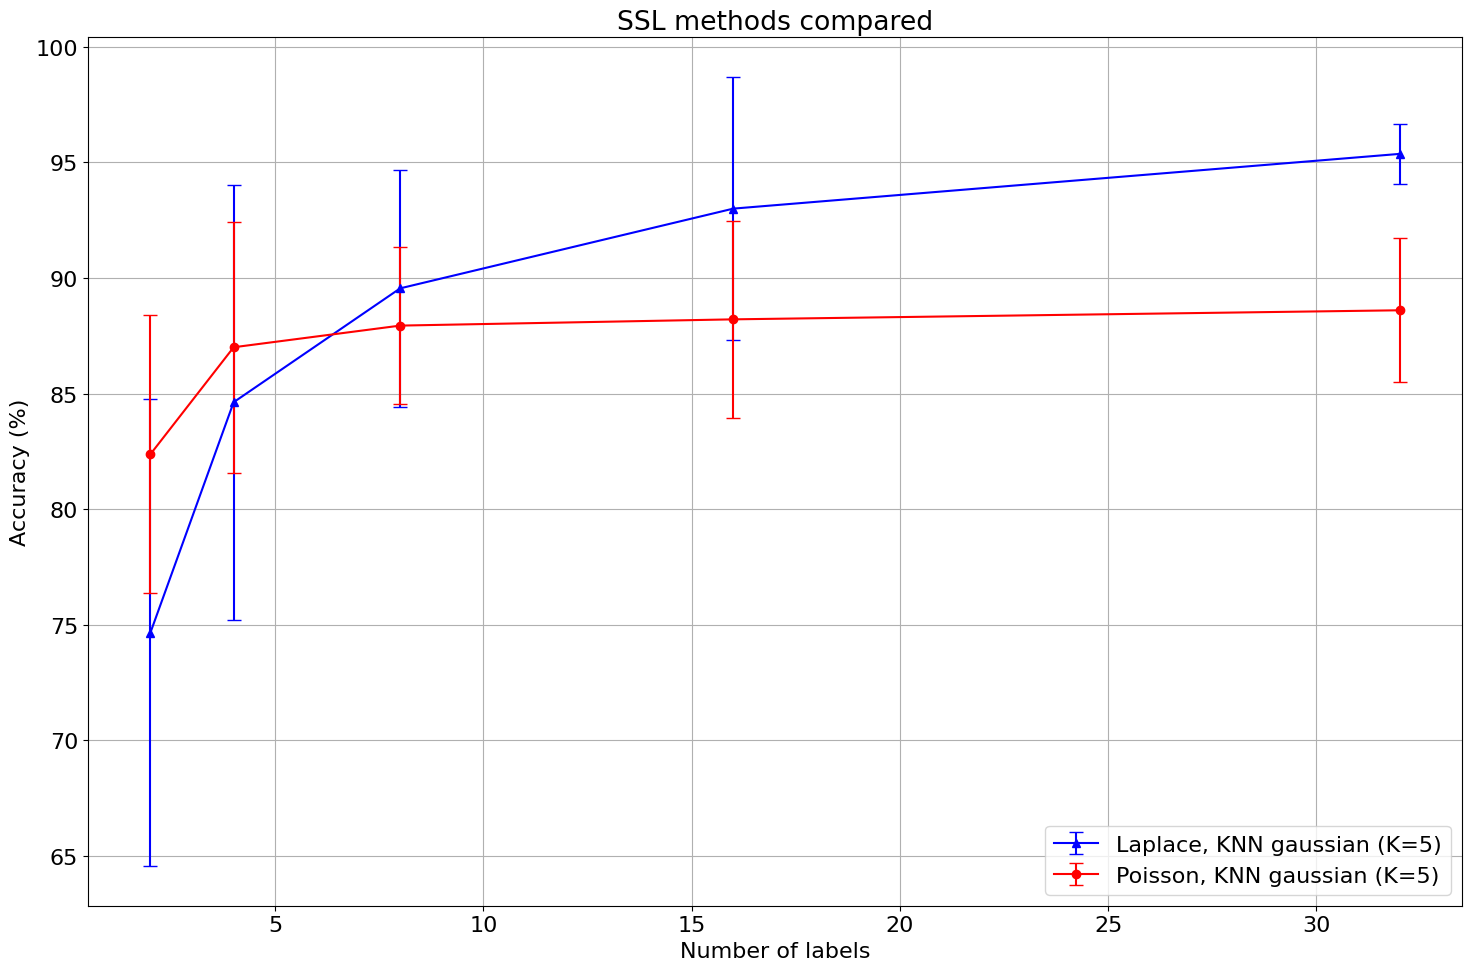
\includegraphics[width=15cm]{Figs/Laplace_Poisson_label_rate.png}
    \caption{Accuracy of Laplace and Poisson learning methods versus the number of labeled datapoints.}
    \label{labelrate}
\end{figure}

\section{Summary and Conclusions}\label{sec:conclusions}

In this report we investigated the integration of Laplacian-based semi-supervised learning methods within the Reproducing Kernel Hilbert Space (RKHS) framework. We examined the theoretical principles of our approach, employing the Probit model, Gaussian Random Fields (GRFs) with the Matérn kernel, and Reproducing Kernel Hilbert Spaces (RKHS) in our methodology.

Utilizing the \textit{graphlearning} Python package, we implemented the Laplace learning and Poisson learning algorithms and compared their performance in a simple binary classification problem. We found that both methods eventually converge to the same classification accuracy, but the Poisson method results in a more decisive classification, with label values propagating further from their source compared to the Laplace method. Our exploration into the impact of varying kernel parameters revealed that the Matérn kernel's smoothness parameter had negligible effect for the specific problem considered, while the length scale parameter had a significant influence on label propagation.

An intriguing result from our study was the contrasting performance of the Laplace and Poisson learning methods in relation to label rates. We found that the Poisson method outperformed the Laplace method for low label rates, as expected from the literature \cite{pmlr-v119-calder20a}, however the Laplace method proved superior when a larger amount of labeled data was available.

In terms of future directions, we would like to further investigate the implementation and performance of additional graph-based SSL algorithms. This intention was previously constrained due to technical difficulties stemming from hardware incompatibilities with the \textit{graphlearning} package for certain algorithms. Additionally, we would like to investigate graphical SSL methodology in more complex domains, such as high-dimensional data or data with non-smooth underlying distributions. These investigations would allow us to examine circumstances under which modifying the smoothness parameter in the Matérn kernel proves beneficial, thereby enhancing our understanding and application of SSL methods.

\section*{Acknowledgements}
Thank you to Bamdad Hosseini for putting together this course!

\bibliographystyle{abbrv}
\bibliography{references} % make sure this matches the .bib file for your corresponding document. You also have to maintain your references in the .bib file 

\end{document}
